\section{Three consistency contracts and their non-implication}
\label{sec:C01:contracts}
The organizing synthesis separates three obligations that are often collapsed into a statement that an agent retained its state. Let $s$ denote a complete implementation state. Its projections include the model-visible context $c(s)$, tool interface $T(s)$, authoritative feasible-action set $F_\alpha(s)$ under current authority epoch $\alpha$, and an effect ledger $\lambda_s$. The ledger maps operation identifiers to typed states such as pending, reconciled success, reconciled failure, and unknown. These are semantic status classes, not unverified model assertions. Let $\Gamma:\mathcal S\to\mathcal S$ be a proposed representation or recovery transformation, with the model parameters, tokenizer, and decoding configuration fixed for the comparison.

For $\epsilon\in[0,1]$, define proposal preservation by
\begin{equation}
 \mathsf P_\epsilon(\Gamma,s)=
 \mathbf1\!\left\{
 \operatorname{TV}\!\left(
 \pi_{\theta,\delta}(\cdot\mid c(s),T(s)),
 \pi_{\theta,\delta}(\cdot\mid c(\Gamma s),T(\Gamma s))
 \right)\leq\epsilon\right\}.
\end{equation}
This compares proposal distributions on a common action alphabet before authorization, including an invalid-proposal symbol where required. It does not establish proposal correctness. Exact preservation is $\mathsf P_0=1$. For a fixed one-step loss $\ell(a)\in[0,L_{\max}]$, $\mathsf P_\epsilon=1$ implies
\begin{equation}
 \left|\mathbb E_{a\sim\pi'}\ell(a)-\mathbb E_{a\sim\pi}\ell(a)\right|
 \leq L_{\max}\epsilon,
\end{equation}
where $\pi$ and $\pi'$ are the two proposal laws in the predicate. This follows from the variational characterization of total variation. It is a one-step guarantee for the specified loss, not an episode-level reliability bound. Conversely, equal task utility need not imply proposal preservation: two distinct actions can have the same consequence. Approximate preservation is therefore a strong diagnostic contract whose necessity depends on the downstream equivalence relation. It cannot be inferred from lexical similarity or unchanged archive bytes. Training adds a distinct obligation: likelihood terms must refer to the information that actually conditioned behavior. Chapter~\ref{ch:C17} treats that likelihood-consistency problem explicitly.

Authority nonexpansion under a transformation that has no new external grant is
\begin{equation}
 \mathsf A(\Gamma,s)=
 \mathbf1\{F_\alpha(\Gamma s)\subseteq F_\alpha(s)\}.
\end{equation}
The authority epoch is held current, not restored from an old conversational snapshot. The subset condition permits conservative loss of permissions; such loss can reduce utility and must be evaluated separately. A legitimate new grant is a different operation with its own approval evidence. The predicate prevents a context rewrite, retrieved instruction, or recovery procedure from silently creating authority.

For a pure representation transformation, effect-state preservation is
\begin{equation}
 \mathsf X(\Gamma,s)=\mathbf1\!\left\{
 \begin{aligned}
 &\operatorname{dom}\lambda_{\Gamma s}=\operatorname{dom}\lambda_s,\\
 &\lambda_{\Gamma s}(u)=\lambda_s(u)
 \quad\forall u\in\operatorname{dom}\lambda_s
 \end{aligned}\right\}.
\end{equation}
The comparison holds external observations fixed. It requires preservation of operation identity and recorded status, including explicit uncertainty. It does not validate an initially incorrect ledger or undo external effects. Reconciliation that acquires new service evidence is a separate transition and can legitimately change an unknown status to confirmed success or failure. A pending or unknown outcome cannot become a proven failure merely because a summary omitted the operation.

The exact contracts $\mathsf P_0$, $\mathsf A$, and $\mathsf X$ are logically independent. Consider a product state with separate context, permission, and ledger coordinates. Changing only a context bit that controls a deterministic proposal violates $\mathsf P_0$ while preserving authority and the ledger. Changing only a permission coordinate from denied to allowed violates $\mathsf A$ while leaving the proposal distribution and ledger unchanged. Changing only a recorded committed outcome to unknown violates $\mathsf X$ while preserving context and permissions. Each construction is a witness that the other two predicates do not imply the third. The claim is not made for the vacuous tolerance $\epsilon=1$. This is an analytical non-implication argument; it is not a claim of a new general theorem about cognition.

The distinction matters in actual mechanisms. Context editing and compaction primarily expose $\mathsf P_\epsilon$ and behavior-conditioning obligations. Privilege monitors expose $\mathsf A$. Checkpoints and effect reconciliation expose $\mathsf X$. Memory updates and model migrations can affect all three. A verifier then tests a specified subset of the required properties; passing that verifier does not establish properties outside its scope. MemoryWalker addresses behavior-time conditioning and Progent privilege control~\cite{j2026memorywalker,corpus250411703}. CyberGym-E2E's vulnerability, proof-of-concept, and patch checks and AgentHorizon's trajectory judgments test different outcome properties; neither demonstrates durable effect-ledger reconstruction~\cite{corpus260604460,corpus261011050}.

The originality of this survey lies in analyzing those boundaries jointly, connecting their assumptions to identifiable implementations, and constructing interventions that distinguish their failures. It does not relabel context editing, rate-distortion analysis, privilege control, or durable execution as newly discovered ideas. Contemporary memory and compression surveys already organize substantial parts of that landscape~\cite{corpus251213564,gou2026selective,colaco2026ratedistortion}. The added question is which contracts survive composition and co-adaptation, and what evidence can falsify that claim. Chapters~\ref{ch:C17}, \ref{ch:C29}, \ref{ch:C32}, and \ref{ch:C33} develop the resulting conditioning, authority, recovery, and integration analyses.


Figure~\ref{fig:C01:contracts} distinguishes the information, authority, and effect boundaries used by these predicates.
\begin{figure}[!htbp]
\centering
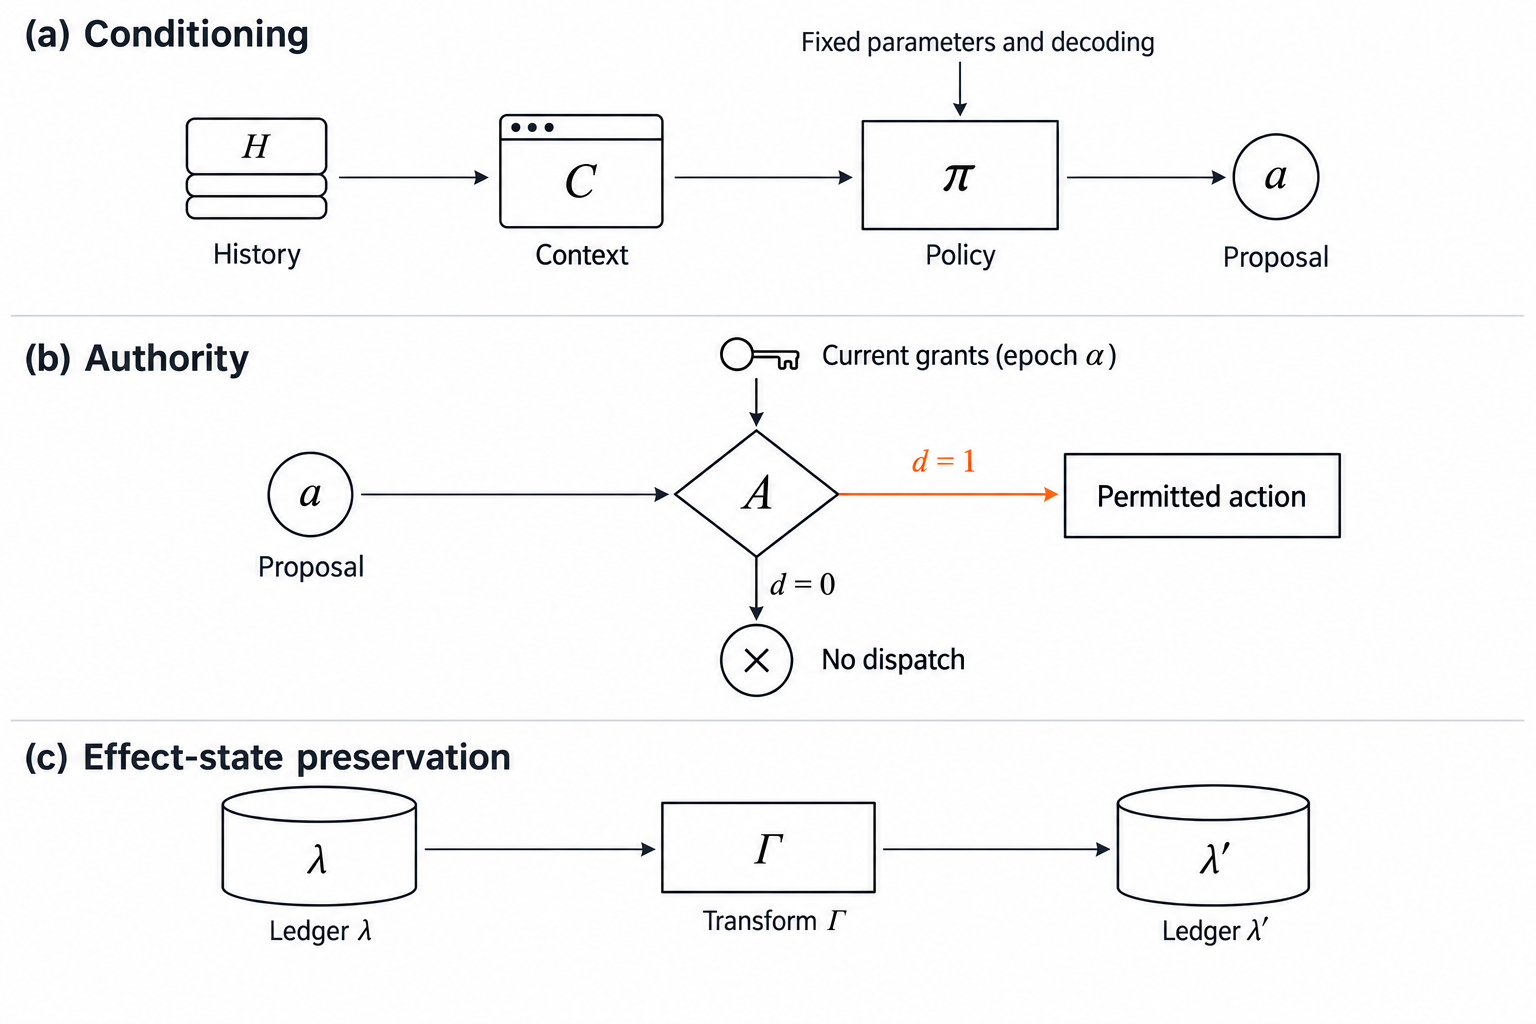
\includegraphics[width=\linewidth]{book/figures/assets/F01v4.png}
\caption{Three separate state contracts. (a) An illustrative history--context--policy path under fixed parameters and decoding; memory and other constructor inputs are omitted. (b) Current grants at authority epoch $\alpha$ gate permitted actions and no dispatch. (c) With $\lambda=\lambda_s$ and $\lambda'=\lambda_{\Gamma s}$, a pure representation transformation preserves operation identities and recorded status, including unknown outcomes. Reconciliation with new service evidence is a different transition. The schematic does not establish task correctness.}
\label{fig:C01:contracts}
\end{figure}

\subsection{From preservation contracts to corrective evidence}
\label{sec:C01:operationalcontracts}
A state transformation can preserve every proposal, permission, and ledger entry while preserving a wrong policy or an incorrect historical record. The three contracts therefore govern transformation integrity; task acceptance requires additional observed evidence. An operational implementation should return scoped verdicts and identify which evidence can resolve a failed or undecidable check. Merely adding a verifier whose output is always accepted would leave this distinction empty.

Let $\mathfrak G\subseteq\{\Gamma:\mathcal S\to\mathcal S\}$ be finite and $z\in\mathcal Z$ an evidence record binding source inputs, versions, current grants, and available receipts. With tolerance $\epsilon$ and authority epoch $\alpha$ fixed, for $i\in\{P,A,X\}$ let $v_i:\mathfrak G\times\mathcal S\times\mathcal Z\to\{0,1,\bot\}$ return failed, passed, or unresolved under a declared checking procedure. Define
\begin{equation}
\label{eq:C01:diagnosticadmission}
\begin{aligned}
 \mathcal D_z(\Gamma,s)
   &=\{i\in\{P,A,X\}:v_i(\Gamma,s;z)\ne1\},\\
 \mathfrak S_z(s)
   &=\{\Gamma s:\Gamma\in\mathfrak G,\ \mathcal D_z(\Gamma,s)=\varnothing\}.
\end{aligned}
\end{equation}
Membership permits advancement under that procedure's scope; admission expires when a governing state version or authority epoch changes. It establishes the mathematical contract only when the checker and its premises justify that inference. In particular, sampled behavioral agreement does not prove equality of proposal distributions. The diagnostic set selects a corrective evidence operation, rather than another undirected reflection.

{\small\setlength{\tabcolsep}{3pt}
\begin{table}[!htbp]
\centering
\caption{Proposed corrective-evidence checks; no experiment is reported.}\label{tab:C01:corrective}
\begin{tabular}{L{16mm}L{45mm}L{51mm}}
\toprule Check & Corrective operation & Required recheck\\\midrule
$P$ & Restore source-bound behavior inputs and transformation lineage. & Declared proposal or decision-preservation property under the fixed configuration.\\
$A$ & Refresh current grants; discard permission inferred from retrieved prose. & Nonexpansion and the exact operation's current authorization.\\
$X$ & Recover operation identities; obtain service evidence when status is unknown. & Ledger continuity; unresolved outcomes remain explicit.\\
\bottomrule
\end{tabular}
\end{table}
}

Effect reconstruction and task validation also need separate outputs. For an operation identifier $u\in\mathcal U$, let $z_E$ and $z_V$ be the corresponding effect-evidence and task-test projections of $z$. Define $\rho:\mathcal U\times\mathcal Z_E\to\{1,0,\bot\}$ as confirmed effect, confirmed absence, or unresolved status under the service contract, and $w:\mathcal U\times\mathcal Z_V\to\{0,1,\bot\}$ as the verdict for a specified task property. Retain
\begin{equation}
\label{eq:C01:effecttaskpair}
 \mathcal Y(u,z)=(\rho(u,z_E),w(u,z_V)).
\end{equation}
Here absence concerns the specified effect, not a claim that no partial effect exists elsewhere. A confirmed upload can contain the wrong artifact; a valid local artifact can coexist with an unknown upload outcome. These observations demand different corrections. Current dispatch authorization remains necessary even after a transformation passes. New service evidence may legitimately revise $\rho$; it must be recorded as reconciliation, not disguised as preservation of the old ledger.

A discriminating study injects one conditioning, grant, or operation-record fault at a time into otherwise matched states. It reports false admission, unresolved decisions, recovery cost, and verified task outcomes separately. No outcome is presumed here: the construction specifies how the chapter's three contracts become diagnosable engineering obligations.
